
\section{Scene Splitting Adaptive Attack}
\label{sec:counter}

\system~ removes uncontrolled randomness in perturbations between similar
frames, thereby disabling adaptive attacks that leverage cross frame pixel
correlations. However, does its own design give rise to new countermeasures?
We carefully considered this question, and discuss what we consider the
strongest possible countermeasure to \system{}. We describe the potential
countermeasure and evaluate its efficacy against \system.

The intuition for the countermeasure is to manipulate the scene
identification process to force a scene break between highly similar
frames. If this can be achieved, then the attacker could obtain two
consecutive (and similar) frames that have been perturbed towards different
targets. They could then apply a version of the pixel-averaging attack to
restore the original, unprotected frames. We call this the scene-splitting
attack, and assume a powerful attacker who can somehow force \system{} to
insert a scene break in the middle of a sequence of similar frames.

\para{The scene splitting attack.} 
We simulate a strong adaptive attack by dividing a single scene from a
video into two subscenes, Scene $S_1$ and $S_2$ each containing $M$ frames. We
use each subscene (Scene$_i$) to generate a target tensor $T_{i}$ with the
aim of maximizing distance between target tensors, which should maximize the
difference between perturbations generated from these targets. 
Now that we have obtained $T_1, T_2$, we apply \system~ to perturb the two
consecutive frames around the bad scene split. Subsequently, we perform a
pixel averaging attack on these two perturbed frames, following the
implementation detailed in \S\ref{sec:eval-limitations}. 

We test our adaptive attack on 20 videos from the Japanese Anime and Video
Game datasets (10 videos from each dataset). We choose these two datasets
because they are best aligned with current threats as explained in
\S\ref{sec:intro}. We limit ourselves to only 10 videos from each category
because of the computation time involved.


\begin{figure}[t]
  \centering
  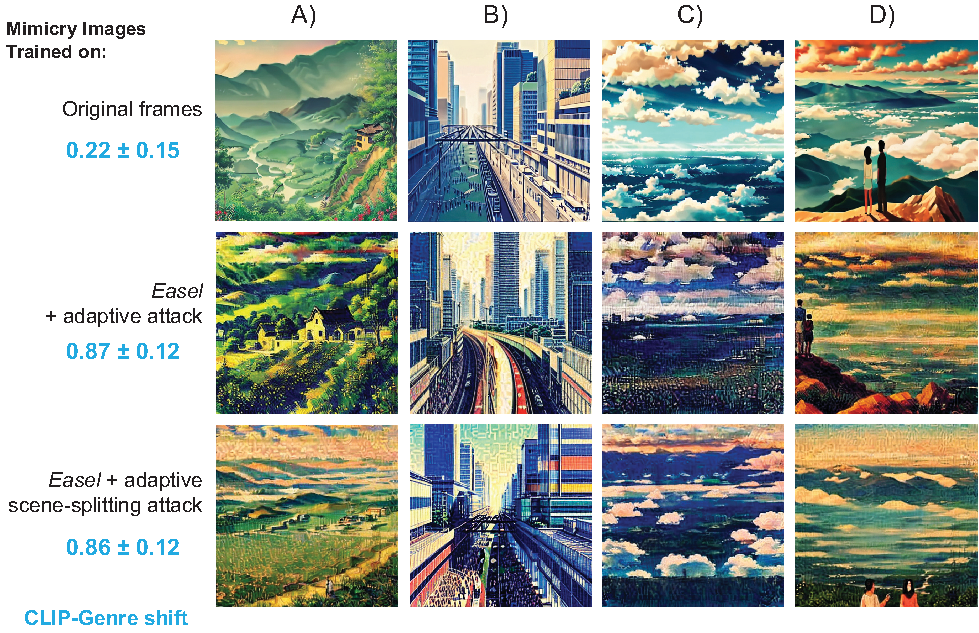
\includegraphics[width=1\columnwidth]{plots/countermeasures-eps-converted-to.pdf}
  \caption{Visual examples of mimicry attempts on Clean frames and frames
    protected by \system~ across the standard Adaptive Attack and the
    Scene-Splitting Adaptive Attack. CLIP-Genre Shift score demonstrates
    robust protection against Mimicry attacks under both adaptive attack
    scenarios.} 
  \label{fig:style-mimicry-ctr}
\end{figure}

\para{\system~ is robust to scene-splitting attack.}
Tables~\ref{tab:countermeasure-loss-score}
and~\ref{tab:countermeasure-pd-score} show results that quantify the
image-level difference between the original frames and the frames produced by
the scene-splitting attack. They show that \system~ is robust to the
scene-splitting attack combined with pixel averaging attacks attempting to
recover original frames. There is only a minimal decrease in $L_2$ norm and
$MPD$ value when \system~ is applied to videos under the new Adaptive
Scene-Splitting Attack. In Figure~\ref{fig:style-mimicry-ctr}, we 
further verify that style mimicry using a combination of
scene-splitting and pixel-averaging is still unsuccessful, through both
visual examples of generated images and associated CLIP-genre shift scores,
which remain unchanged under the scene splitting attack.

\para{Why does the attack fail?} The failure of the scene-splitting attack
makes sense, once we consider its limitations. Regardless of where the
attacker forces a new scene break, frames inside the two new scenes ($S_1$
and $S_2$) are bounded in their maximum difference from each other. Thus the
two source frames for $S_1$ and $S_2$ (each computed as an average of frames
in the scene) is also bounded in their dissimilarity. Thus, it is likely
their resulting target tensors, and consequently the perturbations generated
from them, are also small. This intuition holds even if the attacker could
break a single long scene into several scenes of their choosing.

  \begin{table}[t]
    \centering
      \resizebox{0.5\textwidth}{!}{
      \centering
  \begin{tabular}{c|ccc}
    & Naive         & \multicolumn{1}{c}{\begin{tabular}[c]{@{}c@{}}\system\\ + Adaptive Attack\end{tabular}} & \multicolumn{1}{c}{\begin{tabular}[c]{@{}c@{}}\system~  + Adaptive \\ Scene-Splitting Attack\end{tabular}} \\ \hline
    Video Game     & 405.38 $\pm$ 19.43 & 421.21 $\pm$ 25.52 & 394.80 $\pm$ 25.16       \\
    Japanese Anime & 396.76 $\pm$ 19.05 & 406.43 $\pm$ 24.07 & 387.06 $\pm$ 23.98
\end{tabular}
    }\caption{Latent $L_2$ norm between original and perturbed frames across Video Games and Japanese Anime datasets. Demonstrates Scene-Splitting Adaptive Attack is not able to significantly reduce protection \system~ offers.}
  \label{tab:countermeasure-loss-score}
  \end{table}

  \begin{table}[t]
    \centering
      \resizebox{0.5\textwidth}{!}{
      \centering
  \begin{tabular}{c|ccc}
    & Naive         & \multicolumn{1}{c}{\begin{tabular}[c]{@{}c@{}}\system\\ + Adaptive Attack\end{tabular}} & \multicolumn{1}{c}{\begin{tabular}[c]{@{}c@{}}\system~  + Adaptive \\ Scene-Splitting Attack\end{tabular}} \\ \hline
    Video Game     & 111.58 $\pm$ 12.38 & 107.42 $\pm$ 13.47 & 100.28 $\pm$ 11.81 \\
    Japanese Anime & 112.66 $\pm$ 11.05 & 108.57 $\pm$ 12.59 & 102.02 $\pm$ 11.43       
\end{tabular}
    }\caption{MPD between original and perturbed frames across Video Games and Japanese Anime datasets. Demonstrates Scene-Splitting Adaptive Attack is not able to significantly reduce protection \system~ offers.}
  \label{tab:countermeasure-pd-score}
  \end{table}

